\chapter{Results}
\label{chp4}

\paragraph{ }In this chapter all results obtained from analysing the data and running the anomaly detection algorithms will be presented. 

\section{Beam Displacement Over Time}

\begin{figure}[!b]
	\begin{minipage}[b]{0.475\linewidth}
		\centering
		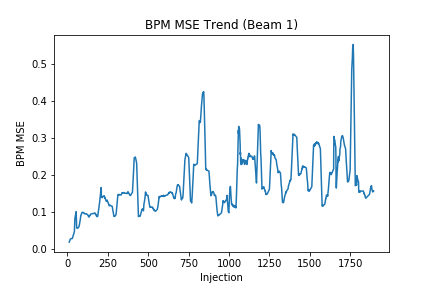
\includegraphics[width=\textwidth]{BPM_MSE_Trend_B1}
		\caption[BPM MSE Trend B1]{Trend Component of the BPM MSE for Beam 1}
		\label{fig::BPM_MSE_Trend_B1}
	\end{minipage}	
	\hspace{0.25cm}
	\begin{minipage}[b]{0.475\linewidth}
		\centering
		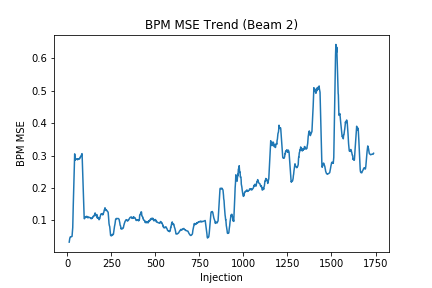
\includegraphics[width=\textwidth]{BPM_MSE_Trend_B2}
		\caption[BPM MSE Trend B2]{Trend Component of the BPM MSE for Beam 2}
		\label{fig::BPM_MSE_Trend_B2}
	\end{minipage}	
\end{figure}

\paragraph{ }When performing the initial analysis on the provided \acs{BPM} data, the \acs{MSE} of the Beam's Position with respect to its initial position in the first injection was calculated (refer to Section \ref{sec::Data_Cleaning_and_Analysis}). A rolling average of the time series points was taken to visualise the trend component. The window size was taken to be 12 since 12 injections are needed to fill the \acs{LHC}. Figures \ref{fig::BPM_MSE_Trend_B1} and \ref{fig::BPM_MSE_Trend_B2} show the trend component for Beam 1 and Beam 2 respectively. Although there's some noise in the data, it is clear from both plots that the Beam's position drifts with time.

\paragraph{ }This result confirms the suspicion that the beam position in the transfer line changes over time, which could have an impact on the injection quality. The cause of this phenomenon is due to ground motion as the slightest movement in one of the \acs{LHC}'s quadrupole magnets can throw off the beam's precision. Thus regular servicing and maintenance of the \acs{LHC} is important to reduce the number of anomalous injections.

\paragraph{ }First order differencing was then done on the data to remove the trend component. The resulting plots can be seen in Figures \ref{fig::BPM_MSE_Diff_B1} and \ref{fig::BPM_MSE_Diff_B2}. From these plots we can conclude that the spikes in the \acs{MSE} values are not cyclic but merely random.

\begin{figure}[!t]
	\begin{minipage}[b]{0.475\linewidth}
		\centering
		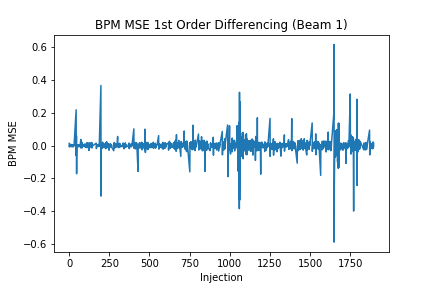
\includegraphics[width=\textwidth]{BPM_MSE_Diff_B1}
		\caption[BPM MSE Differencing B1]{1st Order Differencing for the BPM MSE for Beam 1}
		\label{fig::BPM_MSE_Diff_B1}
	\end{minipage}	
	\hspace{0.25cm}
	\begin{minipage}[b]{0.475\linewidth}
		\centering
		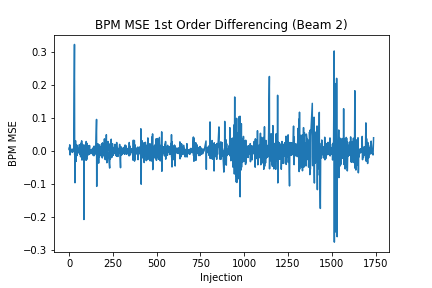
\includegraphics[width=\textwidth]{BPM_MSE_Diff_B2}
		\caption[BPM MSE Differencing B2]{1st Order Differencing for the BPM MSE for Beam 2}
		\label{fig::BPM_MSE_Diff_B2}
	\end{minipage}	
\end{figure}

\section{Anomaly Detection}

\paragraph{ }After running all the algorithms as described in Section \ref{sec::AnomalyDetection}, a total of 131 unique anomalous injections were detected for Beam 1. After manual inspection of each injection by Prof. Valentino, 90 (68.70\%) of these points were found to be actual anomalies. Furthermore, a total of 232 unique anomalous injections were detected for Beam 2, where 134 (57.76\%) of these were found to be actual anomalies. Since we do not know the actual number of anomalous injections that happened over the analysed time period, it was assumed in Chapter \ref{chp5} that these are all the anomalous injections that happened in this time period and  thus the performance of the different algorithms was compared based off of these points.

\subsection{3D \acs{LOF}}

\paragraph{ }Of the  60 injections detected as anomalies by the 3D \acs{LOF} algorithm for Beam 1, 39 of these were found to be actual anomalies (65\%). These detected points can be seen in Figure \ref{fig::3D_results1} where the green points represent the correctly classified injections and the red points represent the false-positives generated. The 2D plots in \ref{fig::3D_results2} and \ref{fig::3D_results3} highlight the nature of these anomalies more clearly. 

\paragraph{ }Of the 98 injections detected as anomalies by the 3D \acs{LOF} algorithm for Beam 2, 45 of these were found to be actual anomalies (45.91\%). These detected points can be seen in Figure \ref{fig::3D_results1_B2}.

\paragraph{ }As can be clearly seen from these plots, performing \acs{LOF} on this 3 dimensional dataset is not sufficient to explain the causes for anomalies as many points that are clearly outliers are not anomalous injections after all. The algorithm still performed reasonably well however and adding more dimensions might improve its performance.

\begin{figure}[h]
	\centering
	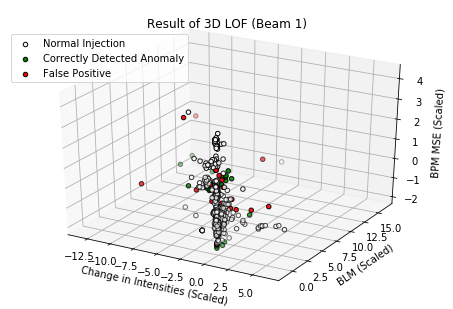
\includegraphics[width=0.8\textwidth]{3D_LOF_Results}
	\caption[3D LoF Results Beam 1]{3D Plot Highlighting Anomalies Detected by the 3D LOF Algorithm for Beam 1}
	\label{fig::3D_results1}
\end{figure}

\begin{figure}[H]
	\centering
	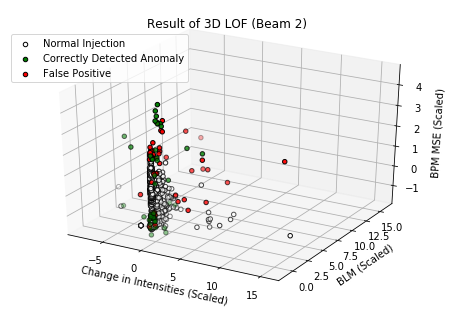
\includegraphics[width=0.8\textwidth]{Beam2_3D_LOF_Results}
	\caption[3D LoF Results Beam 2]{3D Plot Highlighting Anomalies Detected by the 3D LOF Algorithm for Beam 2}
	\label{fig::3D_results1_B2}
\end{figure}    


\begin{figure}[H]
	\centering
	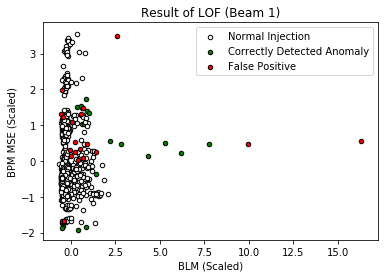
\includegraphics[width=0.8\textwidth]{3D_LOF_BLMBPM}
	\caption[3D LoF Results 2]{Anomalies Detected by the 3D LOF Algorithm}
	\label{fig::3D_results2}
\end{figure}  

\begin{figure}[H]
	\centering
	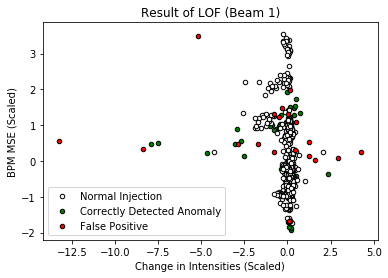
\includegraphics[width=0.8\textwidth]{3D_LOF_ResultsBPMIntensity}
	\caption[3D LoF Results 2]{Anomalies Detected by the 3D LOF Algorithm}
	\label{fig::3D_results3}
\end{figure} 

\subsection{3D \acs{DBSCAN}}

\paragraph{ }The \acs{DBSCAN} algorithm seems to have performed considerably worse than the \acs{LOF} algorithm for 3D data. In fact, only 40 points were detected as anomalous by this algorithm for Beam 1 and only 23 (57.5\%) points were found to be actual anomalous injections. Furthermore, 60 points were detected for Beam 2 where only 28 (46.67\%) were actual anomalies. 

\paragraph{ }These detected points can be seen in Figures \ref{fig::3DBSCAN_results1} and \ref{fig::3DBSCAN_results2} respectively where once again, the green points represent the correctly classified injections and the red points represent the false-positives generated. From these results alone, it was concluded that \acs{LOF} works better for this particular application, thus the full model and the model after performing \acs{PCA} were analysed using \acs{LOF} only.

\begin{figure}[H]
	\centering
	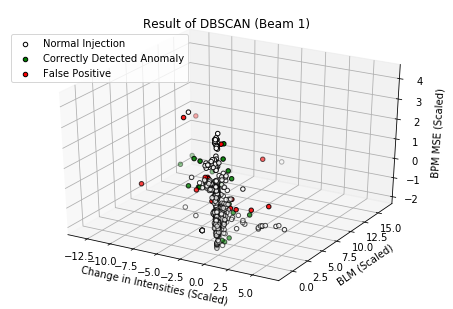
\includegraphics[width=0.8\textwidth]{DBSCAN_Results}
	\caption[3D DBSCAN Results Beam 1]{3D Plot Highlighting Anomalies Detected by the 3D DBSCAN Algorithm for Beam 1}
	\label{fig::3DBSCAN_results1}
\end{figure}

\begin{figure}[H]
	\centering
	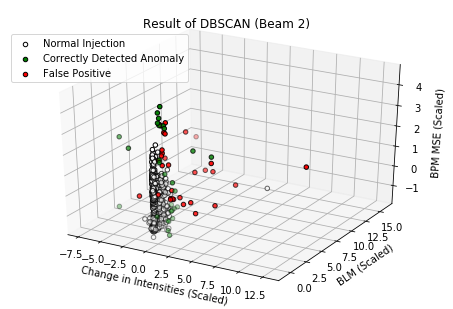
\includegraphics[width=0.8\textwidth]{Beam2_DBSCAN_Results}
	\caption[3D DBSCAN Results Beam 2]{3D Plot Highlighting Anomalies Detected by the 3D DBSCAN Algorithm for Beam 2}
	\label{fig::3DBSCAN_results2}
\end{figure} 

\subsection{Full Model}
\paragraph{ }As expected, running \acs{LOF} on the full dataset seems to have provided better results than when the 3D dataset was used. In particular, of the 64 injections detected as anomalous for Beam 1, 46 (71.88\%) of these were actual anomalies.  96 injections were detected to be anomalous for Beam 2 and 61 (63.54\%) of these were actual anomalies. These results are presented in Figures \ref{fig::Full_results1} and \ref{fig::Full_results2} for Beam 1 and Beam 2 respectively where the same parameters as the 3D data were used in order to be able to visually compare the algorithms' performances.

\paragraph{ }Figures \ref{fig::Full_2D1} and \ref{fig::Full_2D2} are 2D plots which show the nature of these anomalies more clearly, this time for Beam 2. Once again it can be noted that some points which are clearly outliers for the provided dimensions are actually not anomalies. This can be seen in particular for high beam losses. There must be a parameter that's not captured in this model that's causing this phenomenon. Thus, the data was transformed using \acs{PCA} to check if this would improve the performance even more.

\begin{figure}[H]
	\centering
	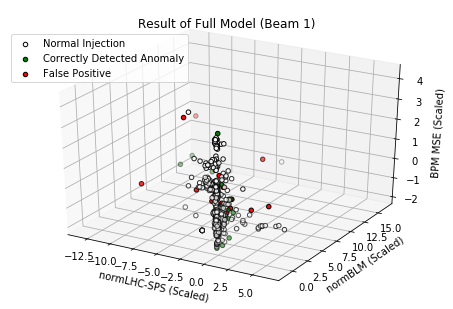
\includegraphics[width=0.8\textwidth]{Full_Results}
	\caption[Full Dataset Results Beam 1]{3D Plot Highlighting Anomalies Detected by the Full LOF Algorithm for Beam 1}
	\label{fig::Full_results1}
\end{figure}

\begin{figure}[H]
	\centering
	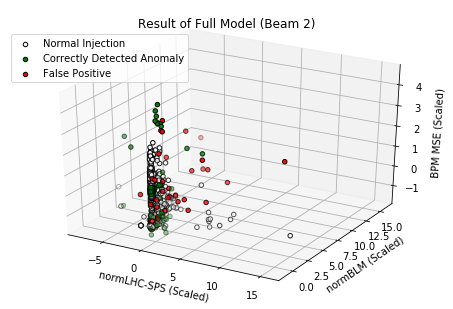
\includegraphics[width=0.8\textwidth]{Beam2_Full_Results}
	\caption[Full Dataset Results Beam 2]{3D Plot Highlighting Anomalies Detected by the Full LOF Algorithm for Beam 2}
	\label{fig::Full_results2}
\end{figure} 

\begin{figure}[H]
	\centering
	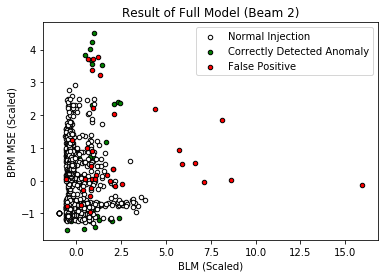
\includegraphics[width=0.8\textwidth]{Beam2_Full_BLMBPM}
	\caption[Full Model BLM/BPM Plot]{Anomalies Detected by the Full LOF Algorithm}
	\label{fig::Full_2D1}
\end{figure}  

\begin{figure}[H]
	\centering
	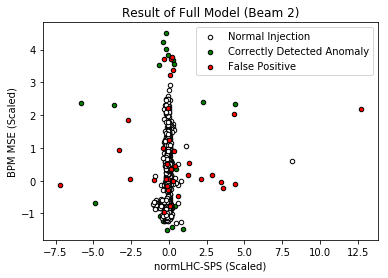
\includegraphics[width=0.8\textwidth]{Beam2_Full_ResultsBPMIntensity}
	\caption[Full Model Intensity/BPM Plot]{Anomalies Detected by the Full LOF Algorithm}
	\label{fig::Full_2D2}
\end{figure} 

\subsection{PCA Model}
\paragraph{ }Although through \acs{PCA}, the transformation of the data led to certain injections (such as those with high losses but still not anomalous) to not be incorrectly classified, the overall performance was similar to that of the full model. Of the 63 injections that were classified as anomalies, 43 (68.25\%) of them were actual anomalies for Beam 1. For Beam 2 however, 115 points were classified as anomalies and 65 (56.52\%) of them were actual anomalies. Figures \ref{fig::PCA_results1} and \ref{fig::PCA_results2} show the nature of the detected anomalies plotted in the same 3 dimensions for Beam 1 and Beam 2 respectively.


\begin{figure}[H]
	\centering
	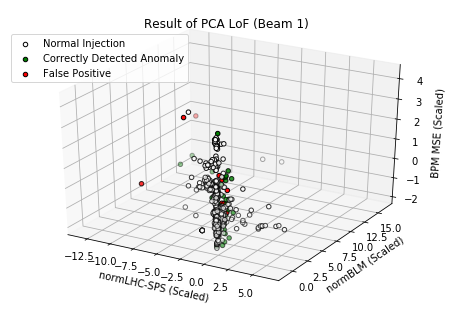
\includegraphics[width=0.8\textwidth]{PCA_Results}
	\caption[PCA Dataset Results Beam 1]{3D Plot Highlighting Anomalies Detected by the Full LOF Algorithm after PCA for Beam 1}
	\label{fig::PCA_results1}
\end{figure}

\begin{figure}[H]
	\centering
	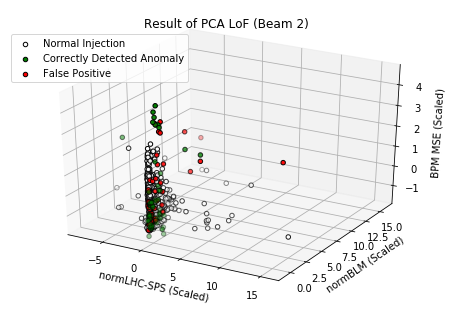
\includegraphics[width=0.8\textwidth]{Beam2_PCA_Results}
	\caption[PCA Dataset Results Beam 2]{3D Plot Highlighting Anomalies Detected by the Full LOF Algorithm after PCA for Beam 2}
	\label{fig::PCA_results2}
\end{figure} 

\section{Nature of Anomalous Injections}
\paragraph{ }One of the purposes of this study is to provide clear visual representations of the anomalies in order for experts to understand more clearly the nature of these anomalies with respect to the studied parameters. Figures \ref{fig::TrueAnomalies} and \ref{fig::TrueAnomalies2} highlight these points.

\begin{figure}[H]
	\centering
	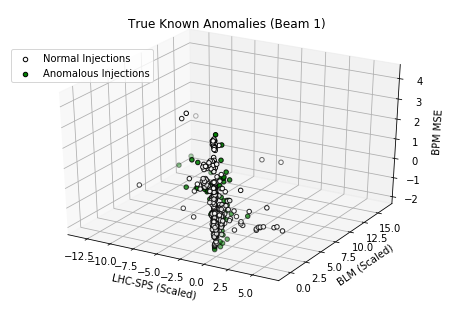
\includegraphics[width=0.7\textwidth]{TrueAnomalies}
	\caption[True Anomalous Injections (Beam 1)]{3D Plot Highlighting the Known Anomalies for Beam 1}
	\label{fig::TrueAnomalies}
\end{figure}

\begin{figure}[H]
	\centering
	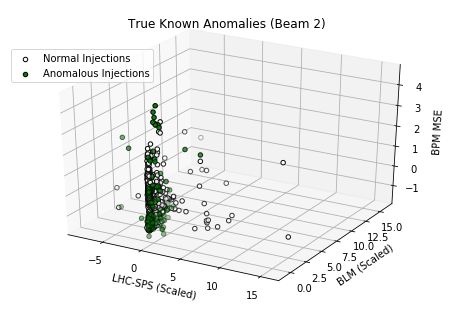
\includegraphics[width=0.7\textwidth]{Beam2_TrueAnomalies}
	\caption[True Anomalous Injections (Beam 2)]{3D Plot Highlighting the Known Anomalies for  Beam 2}
	\label{fig::TrueAnomalies2}
\end{figure} 